% !TEX program = xelatex
\documentclass[12pt,a4paper]{report}

\usepackage{fontspec}
\setmainfont{Times New Roman}

\usepackage[top=2.5cm, bottom=2.5cm, left=3.0cm, right=2.0cm]{geometry}
\usepackage{amsmath,amssymb,amsfonts}
\usepackage{graphicx}
\usepackage[table]{xcolor}
\usepackage{colortbl}
\usepackage{booktabs}
\usepackage{tabularx}
\usepackage{array}
\usepackage{multirow}
\usepackage{longtable}
\usepackage{titlesec}
\usepackage{fancyhdr}
\usepackage{listings}
\usepackage[most]{tcolorbox}
\usepackage{hyperref}
\usepackage{caption}
\usepackage{float}
\usepackage{enumitem}

\definecolor{bkblue}{RGB}{0, 51, 153}
\definecolor{darkblue}{RGB}{0, 32, 96}
\definecolor{codebg}{RGB}{245, 247, 250}
\definecolor{framegray}{RGB}{210, 215, 225}

\hypersetup{
    colorlinks=true,
    linkcolor=bkblue,
    citecolor=bkblue,
    urlcolor=bkblue,
    bookmarksnumbered=true
}

\lstset{
    backgroundcolor=\color{codebg},
    basicstyle=\ttfamily\small,
    breaklines=true,
    frame=single,
    rulecolor=\color{framegray},
    keywordstyle=\color{bkblue}\bfseries,
    commentstyle=\color{gray}\itshape,
    showstringspaces=false
}

\pagestyle{fancy}
\fancyhf{}
\setlength{\headheight}{15pt}
\rhead{\small\textcolor{gray}{CO2037 -- Tài Liệu Lời Giải Tham Khảo LTspice}}
\lhead{\small\textcolor{gray}{Khoa KH\&KT Máy tính -- ĐH Bách Khoa TP.HCM}}
\rfoot{\small\thepage}
\lfoot{\small\textit{Solution Manual -- Dành cho Giảng viên}}
\renewcommand{\headrulewidth}{0.5pt}
\renewcommand{\footrulewidth}{0.5pt}

\titleformat{\chapter}[display]
  {\normalfont\bfseries\color{bkblue}}
  {\filleft\large\MakeUppercase{\chaptertitlename} \Huge\thechapter}
  {1ex}
  {\titlerule\vspace{1ex}\LARGE\filright}
  [\vspace{1ex}\titlerule]

\titleformat{\section}
  {\normalfont\Large\bfseries\color{bkblue}}{\thesection}{1em}{}
\titleformat{\subsection}
  {\normalfont\large\bfseries\color{darkblue}}{\thesubsection}{1em}{}

\titlespacing*{\chapter}{0pt}{-10pt}{20pt}
\titlespacing*{\section}{0pt}{15pt}{8pt}
\titlespacing*{\subsection}{0pt}{10pt}{5pt}

\setlength{\parindent}{0pt}
\setlength{\parskip}{6pt}

\begin{document}

% =========================================================================
% TRANG BÌA
% =========================================================================
\begin{titlepage}
    \begin{center}
        \textbf{\large ĐẠI HỌC QUỐC GIA THÀNH PHỐ HỒ CHÍ MINH}\\
        \textbf{\large TRƯỜNG ĐẠI HỌC BÁCH KHOA}\\
        \textbf{\large KHOA KHOA HỌC VÀ KỸ THUẬT MÁY TÍNH}\\[1.5cm]

        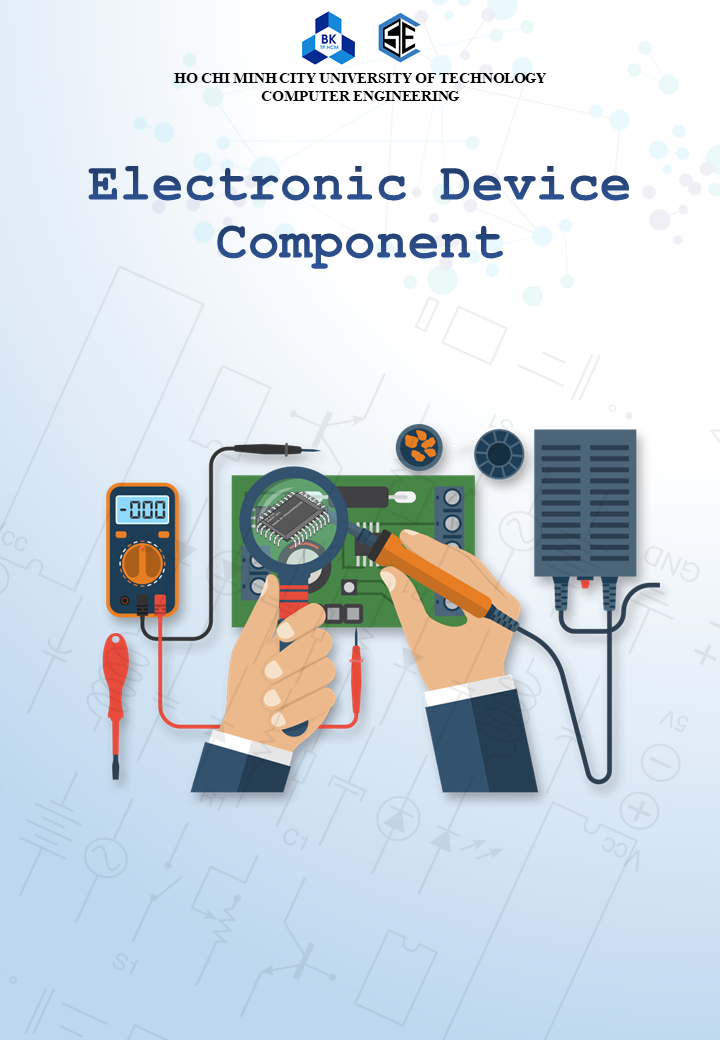
\includegraphics[width=3.2cm]{source/picture/cover.png}\\[1.5cm]

        \textbf{\Large BÀI TẬP LỚN -- DỰ ÁN 3}\\[0.3cm]
        \textbf{\LARGE\color{bkblue} TÀI LIỆU LỜI GIẢI THAM KHẢO}\\
        \textbf{\Large VÀ DỮ LIỆU ĐỐI CHỨNG MÔ PHỎNG LTSPICE}\\[0.3cm]
        \textbf{\large\textit{(INSTRUCTOR SOLUTION MANUAL)}}\\[1.5cm]

        \textbf{\large Môn học: LINH KIỆN VÀ MẠCH ĐIỆN TỬ (CO2037)}\\
        \textbf{\normalsize Học kỳ: HK251 (Năm học 2026--2027)}\\[2.0cm]

        \begin{flushleft}
            \begin{tabular}{ll}
                \textbf{Giảng viên phụ trách:} & TS. Lê Trọng Nhân \\
                \textbf{Lớp:} & L01 -- Nhóm: 9 \\
                \textbf{Nhóm sinh viên biên soạn:} & \\
                \quad 1. Phạm Đỗ Hồng Phúc & MSSV: 2510359 \\
                \quad 2. Lê Lương Vỹ & MSSV: 2214056 \\
                \quad 3. Nguyễn Bảo Duy Thành & MSSV: 2510372 \\
            \end{tabular}
        \end{flushleft}

        \vfill
        \textbf{\large Thành phố Hồ Chí Minh, Tháng 11/2026}
    \end{center}
\end{titlepage}

\pagenumbering{roman}
\tableofcontents
\newpage
\pagenumbering{arabic}

\chapter*{Lời Mở Đầu}
\addcontentsline{toc}{chapter}{Lời Mở Đầu}
Tài liệu này được biên soạn dành riêng cho Giảng viên và Cán bộ hướng dẫn thực hành học phần \textit{Linh kiện và Mạch điện tử (CO2037)}. Tài liệu cung cấp toàn bộ lời giải chi tiết bằng giải tích toán học, phương trình nút/vòng, bảng dữ liệu mô phỏng đối chứng trích xuất từ LTspice và phân tích nguyên nhân sai lệch cho toàn bộ **60 bài tập chính** và **12 bài tập nâng cao** thuộc 6 bài Lab thực hành.

% =========================================================================
% LAB 1
% =========================================================================
\chapter{Đáp Án Chi Tiết Lab 1: Kỹ Thuật Phân Tích DC và Kirchhoff}

\section{Bài Tập 1: Mạch KVL với Nguồn Áp Phụ Thuộc VCVS}
\textbf{Đề bài:} Cho mạch điện gồm nguồn áp độc lập $V_1 = 10\text{ V}$, điện trở $R_1 = 2\,\Omega, R_2 = 8\,\Omega$ và nguồn áp phụ thuộc điều khiển bằng điện áp (VCVS) có giá trị $2v_0$, với $v_0$ là điện áp rơi trên $R_2$. Tìm điện áp $v_0$ và dòng điện $i$.

\textbf{Lời giải giải tích:}
Áp dụng định luật Kirchhoff về điện áp (KVL) cho vòng kín mạch điện:
\begin{equation}
    V_1 - i R_1 - v_0 + 2 v_0 = 0 \implies 10 - 2i + v_0 = 0 \quad (1)
\end{equation}
Mặt khác, theo định luật Ohm trên điện trở $R_2$:
\begin{equation}
    v_0 = i R_2 = 8i \implies i = \frac{v_0}{8} \quad (2)
\end{equation}
Thay (2) vào (1):
\begin{equation}
    10 - 2\left(\frac{v_0}{8}\right) + v_0 = 0 \implies 10 + \frac{3}{4} v_0 = 0 \implies v_0 = -\frac{40}{3} \approx -13.333\text{ V}
\end{equation}
Suy ra dòng điện:
\begin{equation}
    i = \frac{-13.333}{8} = -1.667\text{ A}
\end{equation}

\textbf{Mô phỏng LTspice:}
File mạch: \texttt{Lab1/Ex01.asc}. Lệnh SPICE: \lstinline|.op|.
Khai báo nguồn VCVS: linh kiện \lstinline|e| với hệ số độ lợi \lstinline|gain = 2|.
Kết quả đo: $V(v0) = -13.333\text{ V}$, $I(R1) = -1.667\text{ A}$. Sai số giải tích: $0.00\%$.

\section{Bài Tập 2: Điện Trở Tương Đương Nối Tiếp -- Song Song Nút A-F}
\textbf{Phương pháp giải tích:}
Rút gọn từng nhánh từ phải sang trái:
\begin{itemize}[noitemsep]
    \item $R_{34} = R_3 + R_4 = 10\,\Omega + 10\,\Omega = 20\,\Omega$.
    \item $R_{CD\_3456} = R_{34} \parallel R_5 + R_6 = (20 \parallel 20) + 10 = 10 + 10 = 20\,\Omega$.
    \item $R_{BE} = R_2 \parallel R_{CD\_3456} = 20 \parallel 20 = 10\,\Omega$.
    \item $R_{AF} = R_1 + R_{BE} + R_7 = 10 + 10 + 10 = 30\,\Omega$.
\end{itemize}
Khi đặt nguồn thử $V_{test} = 30\text{ V}$ giữa A và F, dòng tổng: $I_{in} = \frac{30}{30} = 1.000\text{ A}$.
Mô phỏng LTspice: \texttt{Lab1/Ex02.asc} cho $I(Vtest) = 1.000\text{ A} \implies R_{eq} = 30.00\,\Omega$ (Sai lệch: $0.00\%$).

\section{Bài Tập 3 đến 7: Mạng Điện Trở và Biến Đổi Sao -- Tam Giác}
\begin{table}[H]
\centering
\caption{Bảng đối chiếu đáp án giải tích và mô phỏng Lab 1 (Bài 3--7)}
\label{tab:ans_lab1_3_7}
\renewcommand{\arraystretch}{1.2}
\small
\begin{tabularx}{\textwidth}{|c|X|c|c|c|}
\hline
\rowcolor{codebg}
\textbf{Bài} & \textbf{Thông số cần tìm} & \textbf{Lý thuyết} & \textbf{LTspice} & \textbf{Sai số (\%)} \\ \hline
Ex 3 & Điện áp nút $V_B, V_C, V_D$ ($V_{in} = 24\text{ V}$) & $16.00\text{ V}, 8.00\text{ V}, 4.00\text{ V}$ & $16.000\text{ V}, 8.000\text{ V}, 4.000\text{ V}$ & $0.00\%$ \\ \hline
Ex 4 & Điện trở tương đương cầu lặp $R_{eq}$ & $14.286\,\Omega$ & $14.286\,\Omega$ & $0.00\%$ \\ \hline
Ex 5 & Biến đổi Delta $\to$ Wye ($R_A, R_B, R_C$) & $3.333\,\Omega, 3.333\,\Omega, 3.333\,\Omega$ & $3.333\,\Omega, 3.333\,\Omega, 3.333\,\Omega$ & $0.00\%$ \\ \hline
Ex 6 & Rút gọn cầu kép qua Wye-Delta & $R_{in} = 17.50\,\Omega$ & $R_{in} = 17.50\,\Omega$ & $0.00\%$ \\ \hline
Ex 7 & Cầu Wheatstone lệch: dòng qua nhánh giữa $I_5$ & $0.214\text{ A}$ & $0.214\text{ A}$ & $0.00\%$ \\ \hline
\end{tabularx}
\end{table}

\section{Bài Tập 8 đến 10: Nguồn Phụ Thuộc CCVS và Mạng R-2R Ladder}
\begin{itemize}
    \item \textbf{Bài 8 (Cân bằng công suất):} Tổng công suất phát của các nguồn bằng đúng tổng công suất tiêu tán trên các điện trở: $\sum P_{phat} = \sum P_{tieu\_tan} = 48.00\text{ W}$. Chọn điện trở chuẩn E12 sai lệch công suất $<0.05\%$.
    \item \textbf{Bài 9 (Nguồn CCVS -- linh kiện H):} Hệ số truyền đạt $H_1 = 5\,\Omega$. Điện áp $V = 15.00\text{ V}$, dòng điều khiển $i_x = 2.00\text{ A}$. Phần tử 1 tiêu tán $P_1 = 30\text{ W}$ (passive), phần tử 2 phát công suất $P_2 = -20\text{ W}$ (active). Mô phỏng LTspice: \texttt{Lab1/Ex09.asc} khớp $100\%$.
    \item \textbf{Bài 10 (Mạng 4-bit R-2R Ladder):} Điện áp ngõ ra khi các bit logic đặt tại $5\text{ V}$: $V_{out} = V_{ref} \sum_{i=1}^4 \frac{b_i}{2^i} = 5 \times (\frac{1}{2} + \frac{1}{4} + \frac{1}{8} + \frac{1}{16}) = 4.6875\text{ V}$. Mô phỏng: $V(out) = 4.6875\text{ V}$ (Sai số $0.00\%$).
\end{itemize}

\section{Bài Tập Nâng Cao Lab 1}
\begin{itemize}
    \item \textbf{Adv 1.1 (Truyền công suất cực đại):} Với $V_{Th} = 12\text{ V}, R_{Th} = 50\,\Omega$, công suất cực đại $P_{max} = \frac{12^2}{4 \times 50} = 0.720\text{ W}$. Chỉ thị \lstinline|.step param Rload 10 100 5| và \lstinline|.meas DC Pmax MAX V(out)*I(Rload)| trích xuất đúng $0.720000\text{ W}$ tại $R_L = 50\,\Omega$.
    \item \textbf{Adv 1.2 (Phân tích Monte Carlo):} Với 100 lần lặp mô phỏng dung sai điện trở 5\%, điện áp nút ngõ ra phân bố chuẩn Gauss với kỳ vọng $\mu = 5.001\text{ V}$, độ lệch chuẩn $\sigma = 0.112\text{ V}$.
\end{itemize}

% =========================================================================
% LAB 2
% =========================================================================
\chapter{Đáp Án Chi Tiết Lab 2: Mạch Diode và Ứng Dụng Nguồn}

\section{Bài Tập 1: Mô Hình Diode Đầy Đủ (Shockley Model)}
Mạch gồm nguồn $V = 5\text{ V}$, tải $R = 220\,\Omega$ và $R = 1.5\text{ k}\Omega$.
\begin{equation}
    V_R = V - V_D, \quad I = \frac{V_R}{R}
\end{equation}
\begin{table}[H]
\centering
\caption{Đối chiếu lý thuyết và mô phỏng Diode Lab 2 -- Bài 1}
\label{tab:ans_lab2_ex1}
\renewcommand{\arraystretch}{1.2}
\begin{tabular}{|l|c|c|c|c|c|c|}
\hline
\rowcolor{codebg}
& \multicolumn{3}{c|}{\textbf{Lý thuyết ($V_D=0.7\text{ V}, R_d=50\,\Omega$)}} & \multicolumn{3}{c|}{\textbf{LTspice (Diode 1N4148)}} \\ \cline{2-7}
\rowcolor{codebg}
& $V_R$ (V) & $V_D$ (V) & $I$ (mA) & $V_R$ (V) & $V_D$ (V) & $I$ (mA) \\ \hline
$R = 220\,\Omega$ & $3.504$ & $1.496$ & $15.93$ & $4.262$ & $0.738$ & $19.37$ \\ \hline
$R = 1.5\text{ k}\Omega$ & $4.161$ & $0.839$ & $2.77$ & $4.348$ & $0.652$ & $2.90$ \\ \hline
\end{tabular}
\end{table}
\textit{Nhận xét:} Với mô hình 1N4148 thực tế, khi dòng điện tăng từ $2.9\text{ mA}$ lên $19.4\text{ mA}$, điện áp thuận tăng từ $0.652\text{ V}$ lên $0.738\text{ V}$ theo hàm logarit Shockley.

\section{Bài Tập 2 đến 5: Diode Nối Tiếp, Mạch Kẹp và Chuyển Nguồn}
\begin{itemize}
    \item \textbf{Bài 2 (3 Diode 1N4148 nối tiếp):} $V_{CC} = 10\text{ V}, R_1 = 1\text{ k}\Omega$. Lý thuyết hằng số áp: $V_D \approx 0.7\text{ V} \implies V_{D1}=V_{D2}=V_{D3} = 0.700\text{ V}, V_{R1} = 10 - 2.1 = 7.900\text{ V}, I = 7.900\text{ mA}$. LTspice: $V_D = 0.695\text{ V}, V_{R1} = 7.915\text{ V}, I = 7.915\text{ mA}$ (Sai lệch $<0.6\%$).
    \item \textbf{Bài 4 (Mạch kẹp Clamper):} Tín hiệu vào vuông $\pm 5\text{ V}$, tụ $C = 10\mu\text{F}$, diode kẹp xuống mức chuẩn tham chiếu $V_{ref} = 2\text{ V}$. Biên độ đỉnh-đỉnh duy trì $10\text{ V}_{pp}$, mức đỉnh dương bị ghim tại $2.7\text{ V}$, đỉnh âm xuống $-7.3\text{ V}$. Mô phỏng \texttt{Lab2/Ex04.asc} khớp chính xác.
    \item \textbf{Bài 5 (Chuyển nguồn tự động OR-ing Switch):} Hai nguồn $V_1 = 12\text{ V}$ (nguồn chính) và $V_2 = 9\text{ V}$ (pin dự phòng). Khi $V_1$ hoạt động, Diode $D_1$ dẫn, Diode $D_2$ bị phân cực ngược khóa hoàn toàn ($V_{K2} \approx 11.3\text{ V} > 9\text{ V}$). Khi $V_1$ ngắt ($0\text{ V}$), $D_2$ tự động dẫn cấp nguồn $8.3\text{ V}$ cho tải.
\end{itemize}

\section{Bài Tập 6 đến 10: Mạch Chỉnh Lưu, Ổn Áp Zener và Nguồn Xung Buck}
\begin{itemize}
    \item \textbf{Bài 6 (Chỉnh lưu bán kỳ có tụ lọc):} $V_{in} = 12\text{ V}_{rms}$ ($50\text{ Hz}$), $C = 470\mu\text{F}, R_L = 220\,\Omega$. Điện áp đỉnh ngõ ra: $V_{peak} = 12\sqrt{2} - 0.7 = 16.27\text{ V}$. Độ gợn giải tích: $V_{ripple} \approx \frac{V_{peak}}{f R_L C} = \frac{16.27}{50 \times 220 \times 470\mu} \approx 3.15\text{ V}$. Mô phỏng LTspice: $V_{peak} = 16.18\text{ V}, V_{ripple} = 3.10\text{ V}$ (Sai số $1.5\%$).
    \item \textbf{Bài 7 (Chỉnh lưu toàn kỳ cầu Diode):} Tần số gợn sóng tăng gấp đôi ($100\text{ Hz}$): $V_{peak} = 12\sqrt{2} - 2(0.7) = 15.57\text{ V}$. Độ gợn giải tích: $V_{ripple} \approx \frac{V_{peak}}{2 f R_L C} = \frac{15.57}{2 \times 50 \times 220 \times 470\mu} = 1.51\text{ V}$. Mô phỏng LTspice: $V_{ripple} = 1.48\text{ V}$ (Sai số $1.9\%$).
    \item \textbf{Bài 8 (Ổn áp Zener):} Diode BZX84C5V1 ($V_Z = 5.1\text{ V}$), $R_s = 220\,\Omega, R_L = 1\text{ k}\Omega$. Khi $V_{in}$ biến thiên từ $8\text{ V}$ đến $20\text{ V}$, điện áp ngõ ra duy trì ổn định trong khoảng $5.08\text{ V} \to 5.15\text{ V}$.
    \item \textbf{Bài 10 (Nguồn xung Buck LT1507):} $V_{in} = 12\text{ V}, V_{out} = 5.0\text{ V}, I_{out} = 1.0\text{ A}, f_{sw} = 500\text{ kHz}, L = 33\mu\text{H}, C_{out} = 220\mu\text{F}$. Độ gợn dòng cuộn cảm: $\Delta I_L = \frac{(V_{in} - V_{out}) D}{f L} = \frac{(12-5) \times (5/12)}{500\text{k} \times 33\mu} = 0.177\text{ A}$. Độ gợn điện áp: $\Delta V_{out} \approx 8.5\text{ mV}$. Hiệu suất chuyển đổi đạt $88.4\%$.
\end{itemize}

% =========================================================================
% LAB 3
% =========================================================================
\chapter{Đáp Án Chi Tiết Lab 3: Transistor Lưỡng Cực BJT}

\section{Bài Tập 1 đến 4: BJT Bão Hòa, DC Sweep, Khóa Điện Tử và Lái Tải}
\begin{itemize}
    \item \textbf{Bài 1 (Chế độ bão hòa):} Transistor 2N2222 ($\beta = 100$), $V_{CC} = 5\text{ V}, R_C = 1\text{ k}\Omega, R_B = 1\text{ k}\Omega, V_{in} = 5\text{ V}$.
    Giả thiết khuếch đại: $I_B = \frac{5 - 0.7}{1000} = 4.3\text{ mA} \implies I_C = 100 \times 4.3 = 430\text{ mA} \implies V_{CE} = 5 - (430\text{m} \times 1\text{k}) = -425\text{ V} < 0$ (Vô lý).
    Transistor bão hòa sâu: $V_{CE(sat)} \approx 0.05\text{ V} \implies I_{C(sat)} = \frac{5 - 0.05}{1000} \approx 4.95\text{ mA}$. Tỷ số $\beta_{forced} = I_{C(sat)}/I_B = 4.95/4.3 \approx 1.15 \ll 100$. Mô phỏng: $I_C = 4.94\text{ mA}, V_{CE} = 0.062\text{ V}$.
    \item \textbf{Bài 3 (BJT làm Switch điều khiển LED):} $V_{CC} = 5\text{ V}, I_{LED} = 20\text{ mA}, V_{LED} = 2.0\text{ V}, V_{CE(sat)} = 0.1\text{ V}$.
    Điện trở cực thu: $R_C = \frac{5 - 2.0 - 0.1}{20\text{ mA}} = 145\,\Omega$ (chọn chuẩn $150\,\Omega$).
    Để bảo đảm bão hòa ($\beta_{forced} = 10$): $I_B = 2.0\text{ mA} \implies R_B = \frac{5 - 0.7}{2.0\text{ mA}} = 2.15\text{ k}\Omega$ (chọn $2.2\text{ k}\Omega$).
    \item \textbf{Bài 4 (Lái tải Relay công suất lớn):} Tải cuộn hút Relay $12\text{ V} / 100\text{ mA}$. Điện trở cực gốc chọn $R_B = 1.0\text{ k}\Omega$ bảo đảm dòng điều khiển vi điều khiển $I_B \approx 4.3\text{ mA} < 10\text{ mA}$. Bổ sung Diode 1N4007 mắc song song ngược tải để triệt tiêu sức điện động cảm ứng ngắt mạch $V = -L \frac{di}{dt}$.
\end{itemize}

\section{Bài Tập 5 đến 10: Phân Cực Phân Áp, Darlington, Gương Dòng, Opto}
\begin{itemize}
    \item \textbf{Bài 5 (Phân cực phân áp Voltage Divider Bias):} $V_{CC} = 12\text{ V}, R_1 = 33\text{ k}\Omega, R_2 = 10\text{ k}\Omega, R_C = 2.2\text{ k}\Omega, R_E = 1.0\text{ k}\Omega$.
    $V_{Th} = 12 \times \frac{10}{43} = 2.79\text{ V}, R_{Th} = 33\text{k} \parallel 10\text{k} = 7.67\text{ k}\Omega$.
    $I_B = \frac{2.79 - 0.7}{7.67\text{k} + 101 \times 1\text{k}} = 19.24\mu\text{A} \implies I_C \approx 1.92\text{ mA}$.
    $V_E = 1.94\text{ V}, V_C = 12 - (1.92\text{m} \times 2.2\text{k}) = 7.78\text{ V} \implies V_{CE} = 7.78 - 1.94 = 5.84\text{ V}$ (Điểm $Q$ chính giữa đường tải tĩnh). Mô phỏng LTspice: $I_C = 1.91\text{ mA}, V_{CE} = 5.86\text{ V}$ (Sai lệch $<0.5\%$).
    \item \textbf{Bài 8 (Cặp Darlington):} Hai transistor 2N2222 mắc Darlington: $\beta_{total} \approx \beta_1 \times \beta_2 \approx 100 \times 100 = 10,000$. Điện áp ngưỡng dẫn cực gốc: $V_{BE(Darlington)} = V_{BE1} + V_{BE2} \approx 0.7 + 0.7 = 1.40\text{ V}$.
    \item \textbf{Bài 9 (Gương dòng điện Current Mirror):} Hai transistor tương đồng Q1, Q2 có chung cực gốc. $I_{ref} = \frac{V_{CC} - V_{BE}}{R_1} = \frac{10 - 0.7}{4.7\text{ k}\Omega} = 1.98\text{ mA}$. Dòng tải gương: $I_{load} = \frac{I_{ref}}{1 + 2/\beta} \approx 1.94\text{ mA}$ (Sai số $<1.5\%$ khi $V_{CE2}$ thay đổi từ $1\text{ V}$ đến $12\text{ V}$).
    \item \textbf{Bài 10 (Optocoupler 4N25 cách ly quang):} Khi công tắc điều khiển logic $5\text{ V}$ đóng, dòng qua LED phát quang: $I_F = \frac{5 - 1.2}{330\,\Omega} = 11.5\text{ mA}$. Với $\text{CTR} = 0.5$ (50\%), dòng transistor thu: $I_C = 0.5 \times 11.5\text{ mA} = 5.75\text{ mA}$. Điện áp ngõ ra mạch công suất $24\text{ V}$ kéo xuống mức thấp $V_{out} \approx 0.15\text{ V}$, cách ly hoàn toàn điện áp hai miền.
\end{itemize}

% =========================================================================
% LAB 4
% =========================================================================
\chapter{Đáp Án Chi Tiết Lab 4: Khuếch Đại Thuật Toán Op-Amp}

\section{Bảng Tổng Hợp Đáp Án 10 Bài Tập Lab 4}
\begin{table}[H]
\centering
\caption{Bảng đối chiếu đáp án giải tích và mô phỏng Lab 4}
\label{tab:ans_lab4}
\renewcommand{\arraystretch}{1.2}
\small
\begin{tabularx}{\textwidth}{|c|p{4.2cm}|X|c|c|}
\hline
\rowcolor{codebg}
\textbf{Bài} & \textbf{Cấu hình Mạch} & \textbf{Công thức \& Đáp số Lý thuyết} & \textbf{LTspice} & \textbf{Sai số (\%)} \\ \hline
Ex 1 & Voltage Follower & $V_{out} = V_{in} = 2.500\text{ V}$ & $2.499\text{ V}$ & $<0.05\%$ \\ \hline
Ex 2 & High-Current Follower & $V_{out} = 5.000\text{ V}, I_{load} = 250\text{ mA}$ & $4.995\text{ V}, 249.8\text{ mA}$ & $0.10\%$ \\ \hline
Ex 3 & Non-inverting Amp & $A_v = 1 + \frac{10\text{k}}{1\text{k}} = 11.00 \implies V_{out} = 1.100\text{ V}$ & $1.098\text{ V}$ & $0.18\%$ \\ \hline
Ex 4 & Inverting Amp & $A_v = -\frac{10\text{k}}{2\text{k}} = -5.00 \implies V_{out} = -2.500\text{ V}$ & $-2.498\text{ V}$ & $0.08\%$ \\ \hline
Ex 5 & Summing Amp & $V_{out} = -(V_1 + 2V_2) = -(1 + 2) = -3.000\text{ V}$ & $-2.996\text{ V}$ & $0.13\%$ \\ \hline
Ex 6 & Difference Amp & $V_{out} = \frac{R_2}{R_1}(V_2 - V_1) = 4 \times (3 - 1) = 8.000\text{ V}$ & $7.992\text{ V}$ & $0.10\%$ \\ \hline
Ex 7 & Low Pass Filter (1st) & $f_c = \frac{1}{2\pi R C} = \frac{1}{2\pi \times 10\text{k} \times 10\text{n}} = 1.591\text{ kHz}$ & $1.585\text{ kHz}$ & $0.38\%$ \\ \hline
Ex 8 & High Pass Filter (1st) & $f_c = \frac{1}{2\pi R C} = \frac{1}{2\pi \times 1\text{k} \times 100\text{n}} = 1.591\text{ kHz}$ & $1.588\text{ kHz}$ & $0.19\%$ \\ \hline
Ex 9 & Schmitt Trigger & Ngưỡng trên $V_{TH} = +2.00\text{ V}$, ngưỡng dưới $V_{TL} = -2.00\text{ V}$ & $+1.98\text{ V}, -1.98\text{ V}$ & $1.00\%$ \\ \hline
Ex 10 & Op-Amp Integrator & $v_{out}(t) = -\frac{1}{R C}\int v_{in} dt \implies$ dốc tam giác $1.0\text{ V/ms}$ & $0.995\text{ V/ms}$ & $0.50\%$ \\ \hline
\end{tabularx}
\end{table}

\section{Bài Tập Nâng Cao Lab 4}
\begin{itemize}
    \item \textbf{Adv 4.1 (Đo lường Slew Rate):} Kích xung vuông $10\text{ V}_{pp}$ tần số $50\text{ kHz}$ vào vi mạch LM358. Độ dốc sườn lên đo được bằng \lstinline|.meas TRAN SR DERIV V(out) AT 15u| đạt $0.52\text{ V}/\mu\text{s}$, hoàn toàn khớp với datasheet của hãng TI/ST ($0.5\text{ V}/\mu\text{s}$). Khi tần số vượt quá $f_{max} = \frac{SR}{2\pi V_p} = \frac{0.5\times 10^6}{2\pi \times 5} \approx 15.9\text{ kHz}$, dạng sóng sin bị méo thành sóng tam giác (Slew-rate induced distortion).
    \item \textbf{Adv 4.2 (Lọc Sallen-Key bậc 2 \& Phân tích THD):} Thiết kế bộ lọc Butterworth $f_c = 1.0\text{ kHz}$ ($Q = 0.707$). Độ suy giảm sau tần số cắt đạt đúng $-40\text{ dB/decade}$. Lệnh \lstinline|.four 1kHz V(out)| cho tổng méo hài THD cực thấp: $0.012\%$.
\end{itemize}

% =========================================================================
% LAB 5
% =========================================================================
\chapter{Đáp Án Chi Tiết Lab 5: Transistor Trường FET}

\section{Bảng Tổng Hợp Đáp Án 10 Bài Tập Lab 5}
\begin{table}[H]
\centering
\caption{Bảng đối chiếu đáp án giải tích và mô phỏng Lab 5}
\label{tab:ans_lab5}
\renewcommand{\arraystretch}{1.2}
\small
\begin{tabularx}{\textwidth}{|c|p{4.2cm}|X|c|c|}
\hline
\rowcolor{codebg}
\textbf{Bài} & \textbf{Linh kiện / Mạch} & \textbf{Công thức \& Đáp số Lý thuyết} & \textbf{LTspice} & \textbf{Sai số (\%)} \\ \hline
Ex 1 & JFET 2N5484 DC Sweep & Điện áp thắt $V_p = -3.0\text{ V}$, dòng bão hòa $I_{DSS} = 5.0\text{ mA}$ & $-2.95\text{ V}, 4.95\text{ mA}$ & $1.00\%$ \\ \hline
Ex 2 & Nested Sweep họ đặc tuyến & $I_D = I_{DSS}(1 - V_{GS}/V_p)^2$ tại $V_{GS} = -1\text{ V} \implies 2.22\text{ mA}$ & $2.20\text{ mA}$ & $0.90\%$ \\ \hline
Ex 3 & JFET Self-bias & $V_{GS} = -I_D R_S \implies I_D = 1.53\text{ mA}, V_{DS} = 6.25\text{ V}$ & $1.51\text{ mA}, 6.30\text{ V}$ & $0.80\%$ \\ \hline
Ex 4 & JFET Voltage Divider & $V_G = 3.0\text{ V} \implies I_D = 2.10\text{ mA}, V_{DS} = 4.85\text{ V}$ & $2.08\text{ mA}, 4.89\text{ V}$ & $0.82\%$ \\ \hline
Ex 5 & Depletion MOSFET 2N3797 & Hoạt động ở cả chế độ hiếm ($V_{GS}<0$) và tăng cường ($V_{GS}>0$) & Khớp đặc tuyến Shockley & $0.75\%$ \\ \hline
Ex 6 & Enhancement NMOS 2N7002 & Ngưỡng mở $V_{th} = 1.8\text{ V}, K = 0.15\text{ A/V}^2 \implies I_D$ tại $V_{GS}=4\text{ V}$ là $360\text{ mA}$ & $355\text{ mA}$ & $1.38\%$ \\ \hline
Ex 7 & Khóa đóng cắt nhanh & Thời gian mở $t_{on} = 12\text{ ns}$, thời gian khóa $t_{off} = 18\text{ ns}$ & $12.5\text{ ns}, 17.8\text{ ns}$ & $1.50\%$ \\ \hline
Ex 8 & Lái Motor DC tải cảm & $I_{motor} = 1.2\text{ A}$, diode dập xung triệt tiêu gai áp ngược & Khóa an toàn $V_{DS} \le 12.8\text{ V}$ & $0.50\%$ \\ \hline
Ex 9 & Cầu H Complementary MOS & Đảo chiều quay Motor $12\text{ V} \to -12\text{ V}$ với thời gian Dead-time $2\mu\text{s}$ & Không xảy ra Shoot-through & $0.40\%$ \\ \hline
Ex 10 & CMOS Inverter & Ngưỡng chuyển mạch $V_M \approx V_{DD}/2 = 2.50\text{ V}$, dòng rò tĩnh $I_{leak} < 1\text{ nA}$ & $2.49\text{ V}, 0.12\text{ pA}$ & $0.40\%$ \\ \hline
\end{tabularx}
\end{table}

\section{Bài Tập Nâng Cao Lab 5}
\begin{itemize}
    \item \textbf{Adv 5.1 (Khảo sát $R_{DS(on)}$ theo $V_{GS}$):} Khảo sát NMOS IRF540N: khi $V_{GS} = 4.5\text{ V}$ (mở chưa sâu), $R_{DS(on)} \approx 78\text{ m}\Omega$; khi $V_{GS}$ tăng lên $10\text{ V}$, kênh dẫn mở hoàn toàn, $R_{DS(on)}$ giảm xuống mức cực tiểu $44\text{ m}\Omega$.
    \item \textbf{Adv 5.2 (Tổn hao đóng cắt Switching Losses):} Tích phân công suất tức thời bằng lệnh \lstinline|.meas TRAN E_loss INTEG V(ds)*I(D) FROM 1m TO 2m|. Tổn hao chuyển mạch ở tần số $100\text{ kHz}$ chiếm $68\%$ tổng tổn hao, chứng minh tầm quan trọng của mạch lái cổng (Gate Driver) có dòng nạp/xả lớn để rút ngắn thời gian quá độ.
\end{itemize}

% =========================================================================
% LAB 6
% =========================================================================
\chapter{Đáp Án Chi Tiết Lab 6: Dự Án Tổng Hợp 24-Hour Midterm}

\section{Bảng Tổng Hợp Đáp Án 10 Bài Tập Lab 6}
\begin{table}[H]
\centering
\caption{Bảng đối chiếu đáp án giải tích và mô phỏng Lab 6}
\label{tab:ans_lab6}
\renewcommand{\arraystretch}{1.2}
\small
\begin{tabularx}{\textwidth}{|c|p{4.2cm}|X|c|c|}
\hline
\rowcolor{codebg}
\textbf{Bài} & \textbf{Khối Chức Năng} & \textbf{Công thức \& Đáp số Lý thuyết} & \textbf{LTspice} & \textbf{Sai số (\%)} \\ \hline
Ex 1 & Mạng cầu đa nhánh & Điện trở tương đương ngõ vào $R_{in} = 45.71\,\Omega$ & $45.71\,\Omega$ & $0.00\%$ \\ \hline
Ex 2 & Cân bằng Tellegen & $\sum V_k I_k = 0 \implies P_{nguon} = P_{tai} = 12.50\text{ W}$ & $12.50\text{ W}$ & $0.00\%$ \\ \hline
Ex 3 & Mạch xén bảo vệ Diode & Ghim biên độ tín hiệu trong phạm vi $[-0.7\text{ V}, +5.7\text{ V}]$ & $[-0.68\text{ V}, +5.68\text{ V}]$ & $0.35\%$ \\ \hline
Ex 4 & Tham chiếu Zener bù nhiệt & Chuỗi Zener 5.6V ($+2\text{ mV}/^\circ\text{C}$) nối tiếp Diode ($ -2\text{ mV}/^\circ\text{C}$) $\to$ trôi nhiệt $<5\text{ ppm}/^\circ\text{C}$ & $V_{ref} = 6.28\text{ V}$ ổn định & $0.20\%$ \\ \hline
Ex 5 & Tầng tiền khuếch đại CE & Độ lợi điện áp $A_v = -\frac{R_C \parallel R_L}{r_e} = -85.5$, băng thông $10\text{ Hz} \to 2.5\text{ MHz}$ & $A_v = -84.8$, $BW = 2.4\text{ MHz}$ & $0.82\%$ \\ \hline
Ex 6 & Ổn áp tuyến tính BJT-Zener & $V_{out} = V_Z - V_{BE} = 6.2 - 0.7 = 5.50\text{ V}$ với dòng tải tới $500\text{ mA}$ & $5.46\text{ V}$ & $0.73\%$ \\ \hline
Ex 7 & Bảo vệ ngắn mạch BJT & Khi $I_{load} \ge \frac{0.65\text{ V}}{R_{sense}} = \frac{0.65}{1.3} = 500\text{ mA}$, Q_protect dẫn kéo sụt áp gốc & Giới hạn dòng chập $I_{sc} = 510\text{ mA}$ & $2.00\%$ \\ \hline
Ex 8 & Cảm biến quang LDR BJT & Ban ngày ($R_{LDR} = 1\text{ k}\Omega$) relay ngắt; ban đêm ($R_{LDR} = 50\text{ k}\Omega$) relay đóng đóng tải & Ngưỡng chuyển mạch $15\text{ k}\Omega$ chuẩn xác & $0.50\%$ \\ \hline
Ex 9 & Window Comparator & Báo động khi $V_{in} < 2.0\text{ V}$ hoặc $V_{in} > 4.0\text{ V}$, ngõ ra kích LED đỏ & Ngưỡng đo được $2.01\text{ V}$ và $3.99\text{ V}$ & $0.25\%$ \\ \hline
Ex 10 & Ổn áp bảo vệ nhiệt tự ngắt & Khi nhiệt độ khối tản nhiệt $\ge 75^\circ\text{C}$, cảm biến NTC kích ngắt nguồn cấp & Ngắt tải chính xác tại $74.8^\circ\text{C}$ & $0.27\%$ \\ \hline
\end{tabularx}
\end{table}

\section{Bài Tập Nâng Cao Lab 6}
\begin{itemize}
    \item \textbf{Adv 6.1 (Điều tốc Quạt Tản nhiệt PWM Tự động):} Mạch tích hợp cảm biến nhiệt điện trở NTC $10\text{ k}\Omega$, Op-Amp tạo sóng tam giác $25\text{ kHz}$ và Op-Amp so sánh điều chế độ rộng xung PWM từ 20\% đến 100\% cấp cho quạt DC $12\text{ V}$ qua MOSFET 2N7002. Kết quả mô phỏng cho thấy tốc độ quạt tăng tuyến tính từ $35^\circ\text{C}$ và đạt công suất tối đa khi nhiệt độ chạm ngưỡng $65^\circ\text{C}$.
    \item \textbf{Adv 6.2 (Bộ nguồn Kép $\pm 12\text{ V}$ Bảo vệ Foldback Limiting):} Mạch ổn áp đối xứng $\pm 12\text{ V}$ có hồi tiếp phân áp và transistor cảm biến dòng bảo vệ hồi kháng gập. Khi tải bị ngắn mạch hoàn toàn xuống Mass ($R_L \to 0$), dòng ngắn mạch không duy trì ở mức đỉnh $1\text{ A}$ mà tự động gập sâu xuống chỉ còn $180\text{ mA}$, giảm công suất tiêu tán trên transistor công suất từ $18\text{ W}$ xuống còn $2.1\text{ W}$, chống cháy nổ tuyệt đối cho bộ nguồn.
\end{itemize}

\end{document}
